\chapter{Development of Analytical Approach}

\section{Purpose}
Review a selection of my contributions to the literature that have informed the approach used in this project throughout my tenure as a member of the lab
\begin{enumerate}
 \item Comparative genomics allows the discovery of cis-regulatory elements in mosquitoes
  \begin{itemize}
   \item Use of comparative genomics to discover putative CREs from orthologous promoter regions in mosquitoes that were able to be corelated with bloodmeal associated transcription control
  \end{itemize}
 \item RNA-seq analyses of blood-induced changes in gene expression in the mosquito vector species, Aedes aegypti
  \begin{itemize}
   \item relevance
  \end{itemize}

 \item Strain Variation in the Transcriptome of the Dengue Fever Vector, Aedes aegypti
   \begin{itemize}
   \item relevance
  \end{itemize}
 \item Comparative Transcriptome Analyses of Deltamethrin-Resistant and-Susceptible Anopheles gambiae Mosquitoes from Kenya by RNA-Seq
   \begin{itemize}
   \item relevance
  \end{itemize}
 \item Complex Modulation of the Aedes aegypti Transcriptome in Response to Dengue Virus Infection
   \begin{itemize}
   \item relevance
  \end{itemize}
\end{enumerate}

\section{Comparative genomics allows the discovery of cis-regulatory elements in mosquitoes}


Figure \ref{fig:mosqPhyloTree}


Figure \ref{fig:sieglaff2009_full}



\begin{figure}[hp]

\hfil
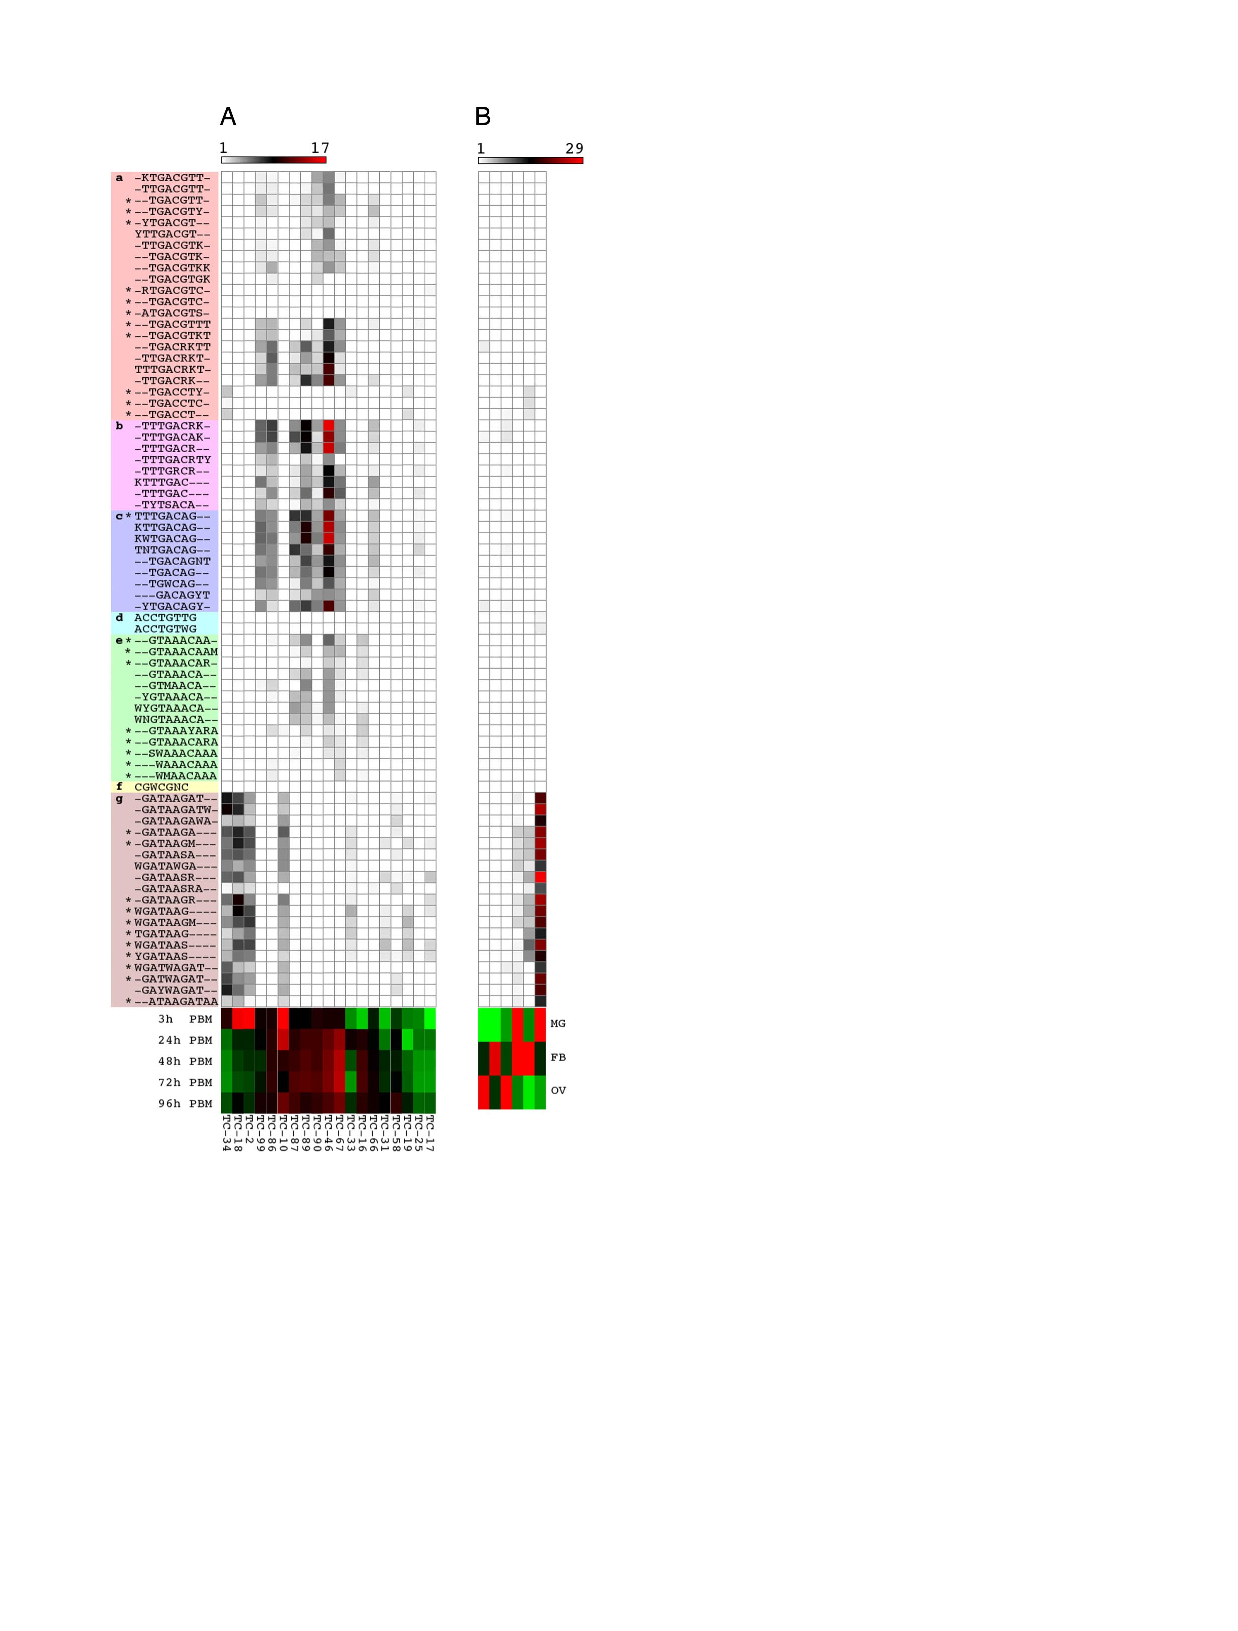
\includegraphics[scale=.95]{figures/figs/sieglaff2009_full.pdf}
\hfil
\caption[Associations of mosquito motifs with gene expression profiles in \Ag]{\bsf{Associations of mosquito motifs with gene expression profiles in \Ag:} \\ \sf
Motif enrichment within (A) 5′-end flanking regions of genes in clusters responsive to blood meal ingestion, and in (B) 5′-end flanking regions of genes in clusters enriched in selected tissues. The significance of motif enrichment is indicated by pseudocolor of -log10 (P-value) determined through hypergeometric statistics, and the median expression profile of each gene cluster is shown below each respective column. Red and green colors represent higher and lower relative mRNA accumulation, respectively. Asterisks (*) indicate a match to a previously described mosquito TFBS. Heatmaps were created with Matrix2png (\CITEME:local-58). FB, fat body; hPBM, hours post blood meal; MG, midgut; OV, ovaries; TC, time course clusters.

Adapted from \cite{Sieglaff2009}}
\label{fig:sieglaff2009_full}
\end{figure}

\begin{figure}[hp]
\centering

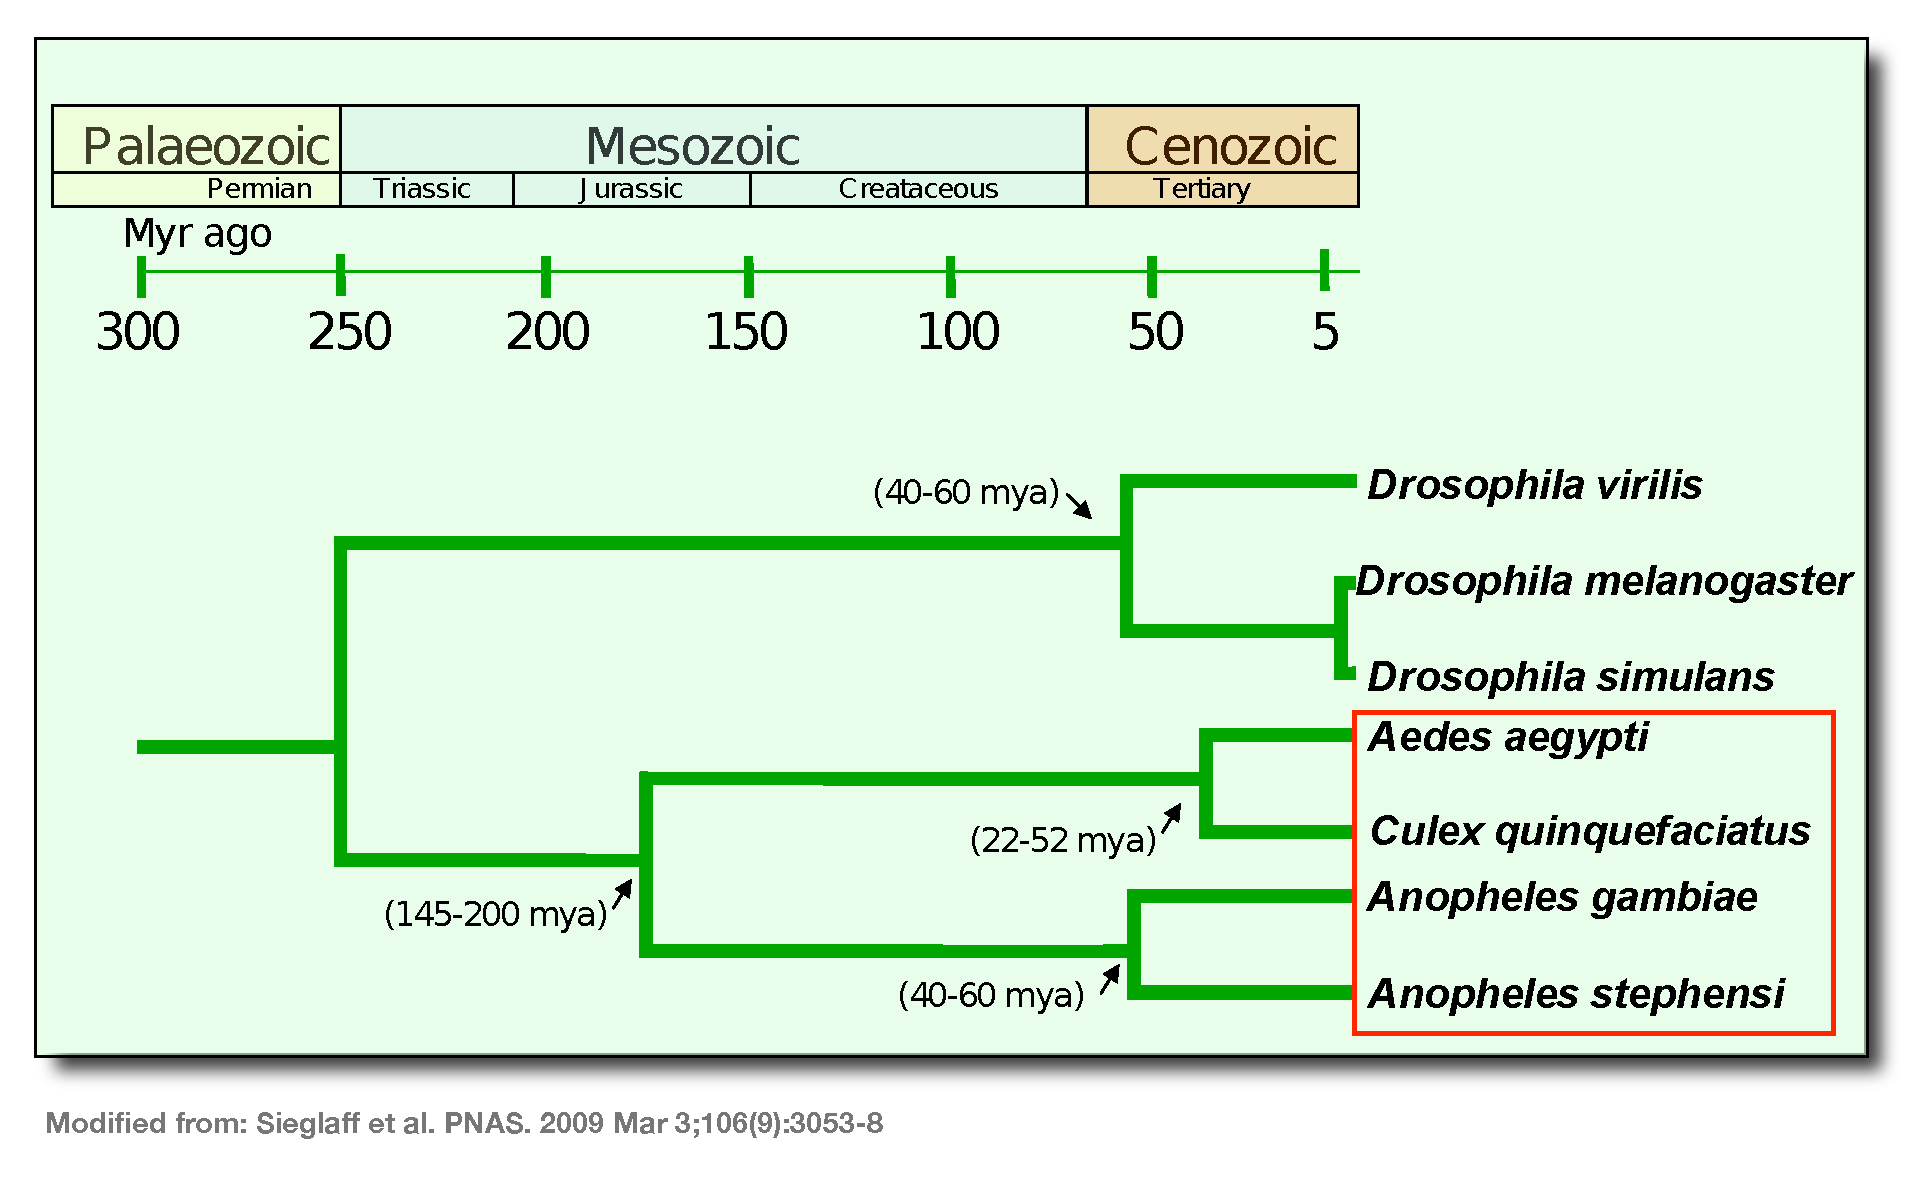
\includegraphics[width=.7\textwidth]{figures/figs/mosqPhyloTree.pdf}

\caption[Phylogenetic relationships between four vector mosquitoes]{\bsf{Phylogenetic relationships between four vector mosquitoes compared with representative \textit{Drosophila} species:} \\ \sf
\dummytext[1]

Adapted from \cite{Sieglaff2009}}
\label{fig:mosqPhyloTree}
\end{figure}


\section{RNA-seq analyses of blood-induced changes in gene expression in the mosquito vector species, Aedes aegypti}

Figure \ref{fig:aedesHMMsplice}


Figure \ref{fig:bonnizoniCREs}


\begin{figure}[hp]
\centering
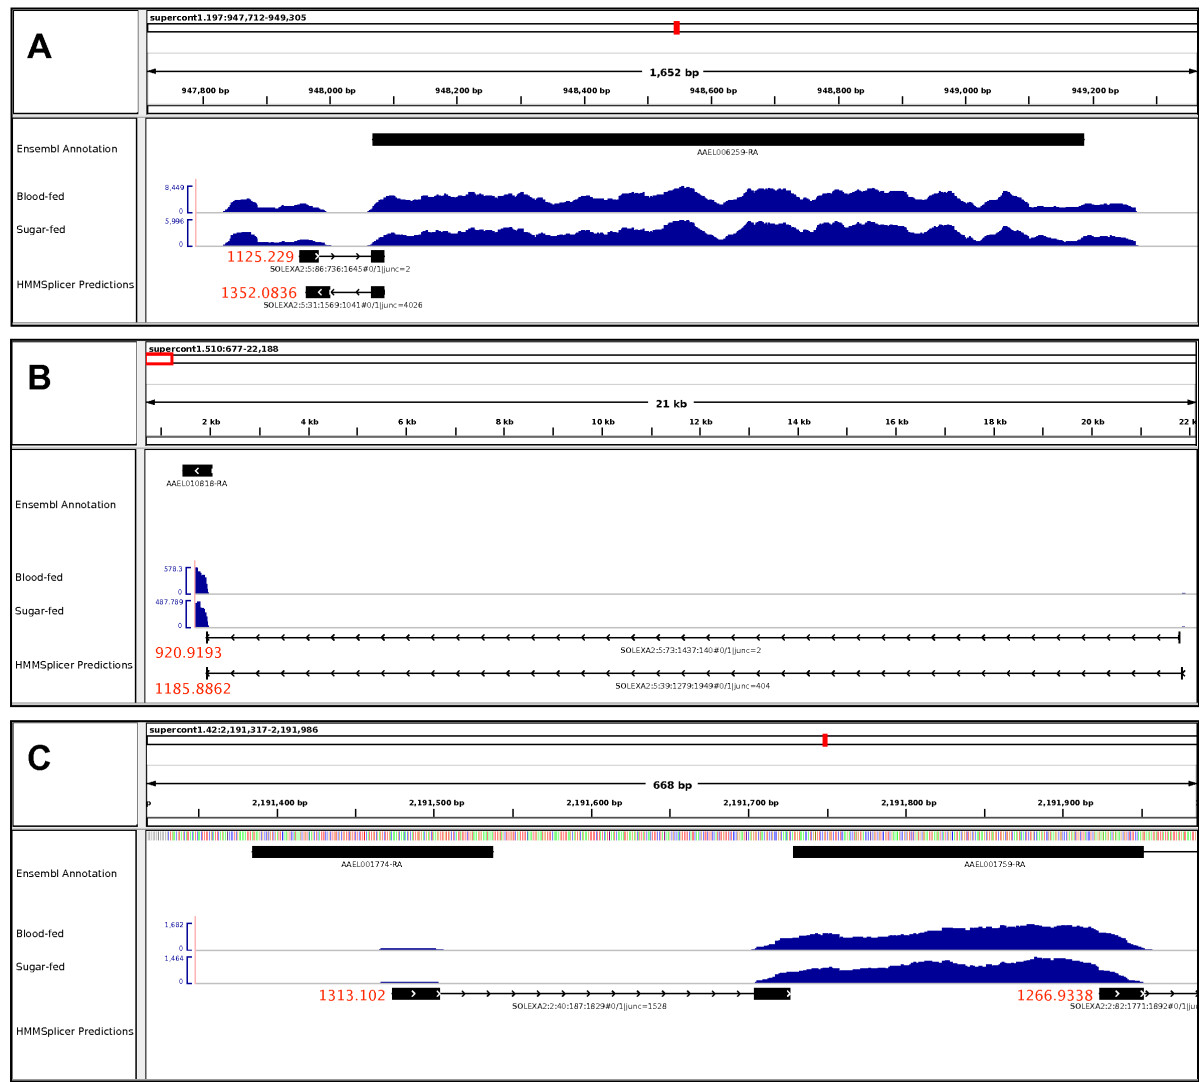
\includegraphics[width=.95\textwidth]{figures/figs/aedesHMMsplice.jpg}

\caption[Examples of amendments to the \Aa\ annotation supported by HMMSplicer results]{\sf \textbf{Examples of amendments to the \Aa\ annotation supported by HMMSplicer results:} Black bars in the top tracks represent the current gene annotations. Blue histograms in the second track represent the non-normalized coverage of RNA-seq reads at each position. The range of the histogram values shown in each view is depicted on the labeled y-axis of each RNA-seq track. Black boxes in the lower track represent splice-site predictions based on the RNA-seq reads using HMMSplicer determined in this study. Each function has a unique identifier listed below and its HMMSplicer score is listed in red. If multiple reads support a single junction, "junc = x" lists the number of supporting reads. This information provides evidence to link two islands of transcription as a single transcription event, therefore, exons of a common mRNA. All predicted junctions shown here also are supported by EST alignments. Genes are (A) AAEL006259; (B) AAEL010818; and (C) AAEL001774 and AAEL001759.

Excerpted from \cite{Bonizzoni2011}}
\label{fig:aedesHMMsplice}
\end{figure}

\begin{figure}[hp]

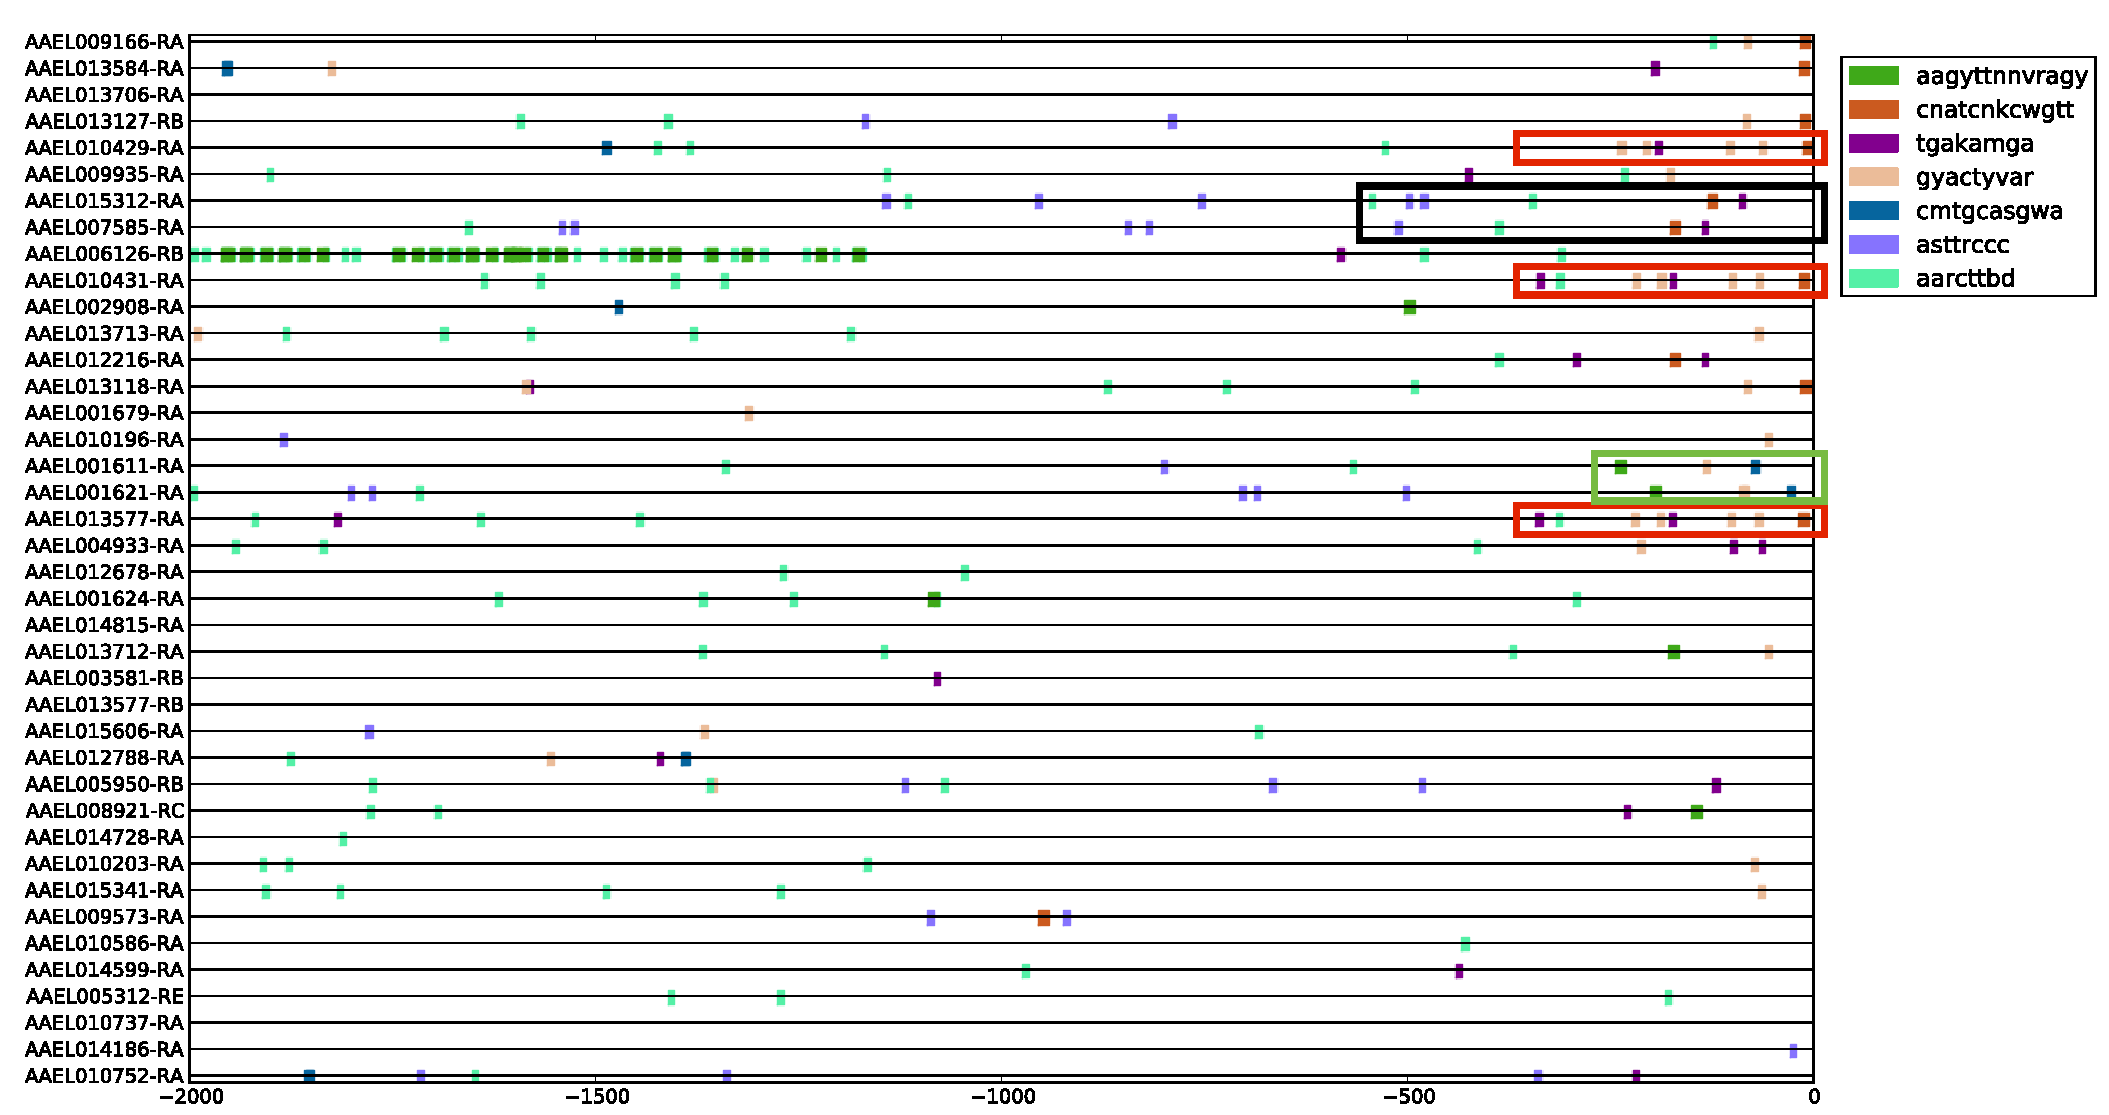
\includegraphics[width=.9\textwidth]{figures/figs/bonnizoniCREs.pdf}

\caption[Motif map of putative CREs from transcripts detected only in bloodfed female \Aa]{\sf \textbf{Motif map of putative CREs discovered by SCOPE using transcripts detected significantly only in bloodfed female \Aa:} Locations of representative SCOPE-derived CRE motifs in the 2000 bp upstream of the annotated translational start site in the 40 transcripts detected significantly only in bloodfed females. Transcript names on the left are ordered from most (top) to least (bottom) abundant.  Candidate CRMs are highlighted in like-colored rectangles.

Adapted from \cite{Bonizzoni2011}}
\label{fig:bonnizoniCREs}
\end{figure}

\section{Strain Variation in the Transcriptome of the Dengue Fever Vector, Aedes aegypti}

Figure \ref{fig:aa-diff-paralogs}

\begin{figure}[h]

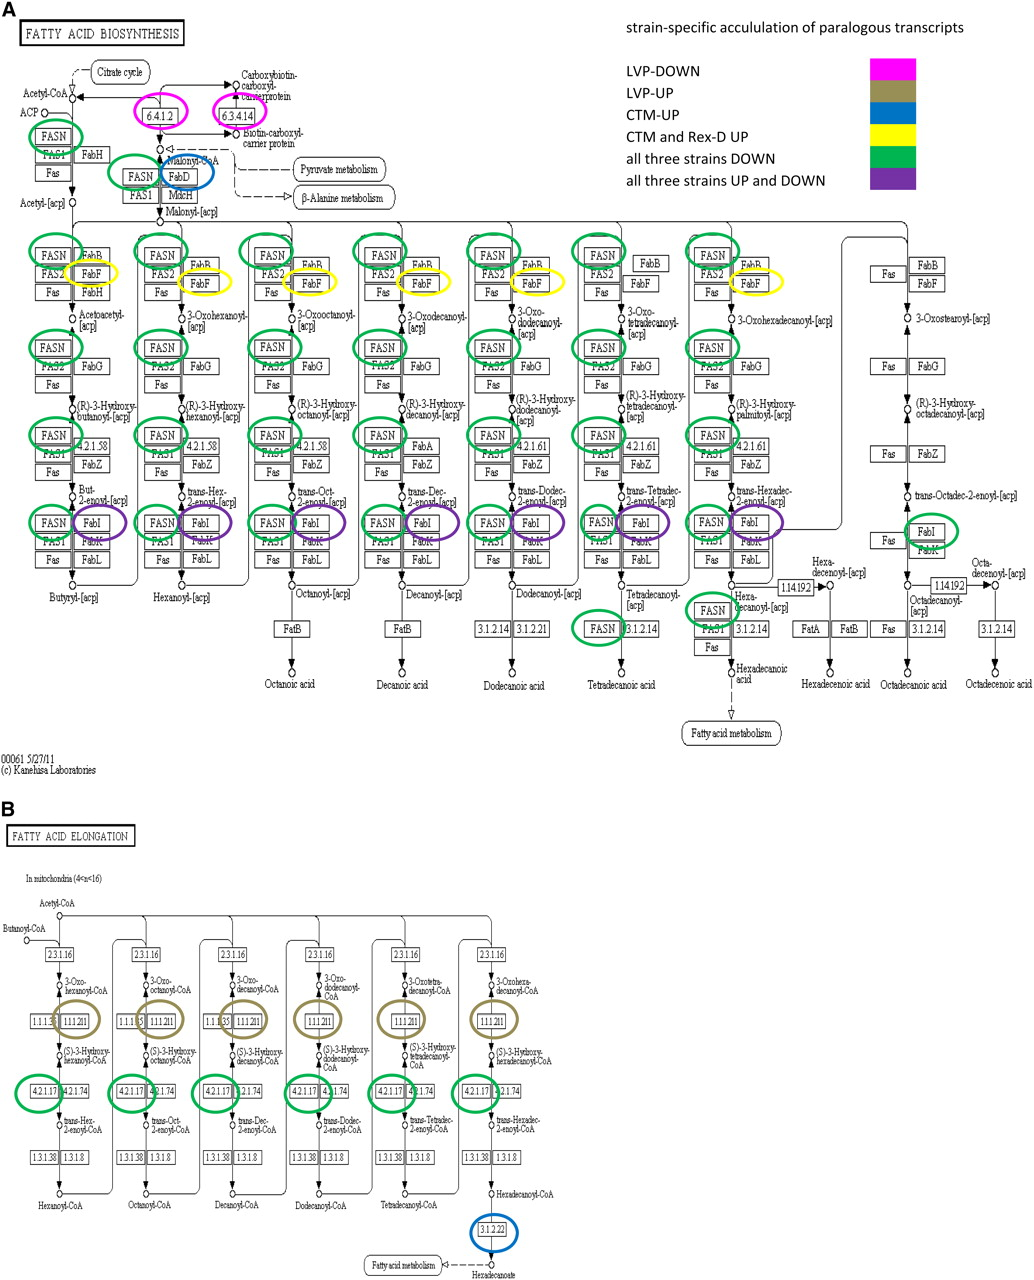
\includegraphics[width=.9\textwidth]{figures/figs/aa-diff-paralogs.jpg}

\caption[Fatty acid biosynthesis and elongation in mitochondria]{\sf \textbf{Fatty acid biosynthesis and elongation in mitochondria:} Proteins corresponding to transcripts accumulated in a strain-specific manner are circled in a color corresponding to the strain and condition defined in the legend (panels A and B).

Excerpted from \cite{bonizzoni2012strain}}
\label{fig:aa-diff-paralogs}
\end{figure}



\section{Complex modulation of the Aedes aegypti transcriptome in response to dengue virus infection}

Figure \ref{fig:bonizzoni2012complex-cre}

\begin{figure}[hp]
\centering

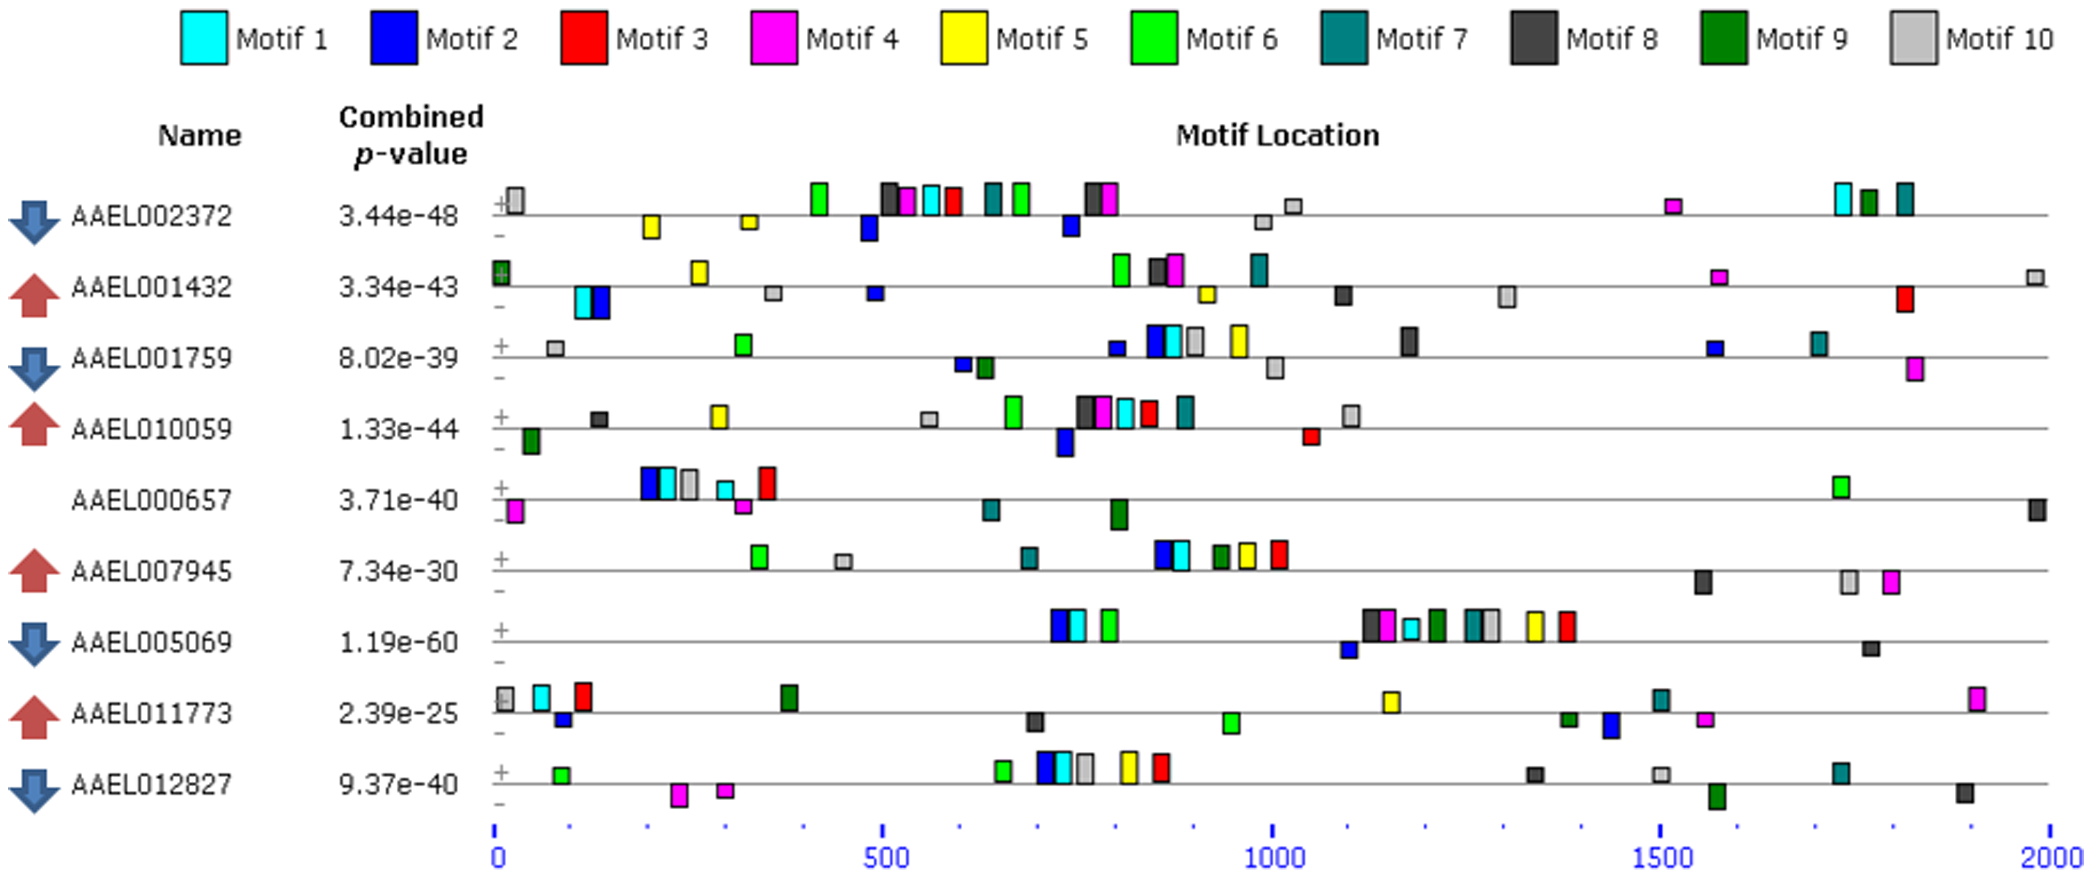
\includegraphics[width=.99\textwidth]{figures/figs/bonizzoni2012complex-cre.png}

\caption[MEME analysis of nine genes with \texorpdfstring{FPKM\textsubscript{DENVI}}{FPKM DENVI} ≥ 100 in carcasses and salivary glands at 14 dpi]{\sf \textbf{MEME analysis of nine genes with \texorpdfstring{FPKM\textsubscript{DENVI}}{FPKM DENVI} ≥ 100 in carcasses and salivary glands at 14 dpi} These genes also were identified with transcripts exhibiting significant differential accumulation in analyses of salivary gland samples of the Liverpool strain infected with DEV2 Thailand 16881 [26]. Colored boxes represent individual putative CREs and their locations in promoters of each gene. Red and blue arrows adjacent to Ensembl Gene ID indicate those genes whose transcripts were detected previously as more or less abundant following DENV infection [26]. Distances in base-pairs are provided below the schematic of each gene.
doi:10.1371/journal.pone.0050512.g004

Excerpted from \cite{bonizzoni2012complex}}
\label{fig:bonizzoni2012complex-cre}
\end{figure}

% \texorpdfstring{FPKM\textsubscript{DENVI}}{FPKM DENVI}


\section{\texorpdfstring{like\textsubscript{this}}{like this}}

%%% Local Variables: ***
%%% mode: latex ***
%%% TeX-master: "thesis.tex" ***
%%% End: ***
